\documentclass[11pt,letterpaper]{article}

\usepackage[utf8]{inputenc}
\usepackage[margin=0.86in,headheight=14pt,headsep=14pt,bottom=0.86in]{geometry}
\usepackage{lmodern}
\usepackage{microtype}
\usepackage{amsmath,amssymb}
\usepackage{graphicx}
\usepackage{booktabs}
\usepackage{tabularx}
\usepackage{fancyhdr}
\usepackage{xcolor}
\usepackage{hyperref}
\usepackage{enumitem}
\usepackage{lastpage}

% Hyperref setup
\hypersetup{
    colorlinks=true,
    linkcolor=black,
    citecolor=black,
    urlcolor=blue
}

% Page style setup
\pagestyle{fancy}
\fancyhf{}
\fancyhead[L]{\small Applied Machine Learning \textbar\ Cornell Tech}
\fancyhead[R]{\small Human or AI?}
\fancyfoot[C]{\small Page \thepage\ of \pageref{LastPage}}
\renewcommand{\headrulewidth}{0.4pt}
\renewcommand{\footrulewidth}{0pt}

\setlength{\parindent}{0pt}
\setlength{\parskip}{5pt plus 1pt minus 1pt}

\begin{document}

% -------------------------------------------------------------
% PAGE 1: TITLE & COMPETITION OVERVIEW
% -------------------------------------------------------------
\thispagestyle{empty}

{\small\textbf{CORNELL TECH \textbar\ APPLIED MACHINE LEARNING}}
\vspace{4pt}

{\LARGE\textbf{Human or AI?}}
\vspace{2pt}

{\large Kaggle Competition \& Report Template}
\vspace{4pt}

\textbf{Report Template: TEMPLATE}
\vspace{10pt}

\textbf{Welcome to the competition!} Your task is to build a machine learning classifier that predicts whether a passage was written by a human or generated by an AI model. You will use a labeled training set, an additional unlabeled set, and a held-out Kaggle test set. The aim is not just a high leaderboard score: we want you to compare methods, design careful experiments, understand generalization, and explain what your results actually show.

You are encouraged to try several approaches. A well-tested logistic regression or support vector machine is just as legitimate as a neural network. The project is designed to be approachable on a laptop; a GPU is \textbf{not required} for full credit.

\vspace{8pt}
\begin{tabular}{@{}ll@{}}
\textbf{Team / members} & [Names, NetIDs] \\[3pt]
\textbf{Kaggle team name} & [Team Name] \\[3pt]
\textbf{GitHub PR URL} & [https://github.com/...] \\
\end{tabular}

\vspace{10pt}
{\large\textbf{Your data}}
\vspace{4pt}

\begin{tabularx}{\textwidth}{@{}llp{1.8cm}X@{}}
\toprule
\textbf{File} & \textbf{Rows} & \textbf{Labels} & \textbf{Purpose} \\
\midrule
\texttt{train.csv} & 10,000 & Visible & Supervised model development: 5,000 human (0), 5,000 AI (1) \\
\texttt{unlabeled.csv} & 3,000 & Hidden & Optional input for semi-supervised methods; required experiment \\
\texttt{test.csv} & 3,000 & Hidden & Predict the probability of AI authorship for Kaggle \\
\texttt{train\_starter\_2000.csv} & 2,000 & Visible & Convenient subset of \texttt{train.csv} for quick experiments \\
\bottomrule
\end{tabularx}

\vspace{4pt}
{\footnotesize The starter data is a subset, not 2,000 additional labeled examples. Passages are approximately 75--350 words, with mean length near 210 words.}

\vspace{10pt}
{\large\textbf{How the test set works}}
\vspace{4pt}

The test set mixes familiar and unfamiliar writing domains and AI generators, and includes some adversarially modified AI-written passages. You will \textbf{not} receive labels, source model names, domain labels, or difficulty memberships for individual test examples. Submit a probability in $[0, 1]$ for each test ID, where 1 means AI-generated. Kaggle evaluates submissions using \textbf{area under the ROC curve (AUROC)}. The \textbf{public leaderboard} covers 900 examples (30\%); the \textbf{private leaderboard} covers 2,100 (70\%) and determines the final competition performance score.

\newpage

% -------------------------------------------------------------
% PAGE 2: RUBRIC & INSTRUCTIONS
% -------------------------------------------------------------
{\large\textbf{1. Competition rubric and submission instructions}}
\vspace{4pt}

\begin{tabularx}{0.7\textwidth}{@{}Xr@{}}
\toprule
\textbf{Component} & \textbf{Points} \\
\midrule
Kaggle private leaderboard performance & 25 \\
Model comparison and selection & 15 \\
Effect of training data size & 10 \\
Learning from unlabeled data & 5 \\
Generalization and error analysis & 20 \\
Open-ended improvements and insights & 15 \\
Code submission and GitHub PR history & 10 \\
\midrule
\textbf{Total} & \textbf{100} \\
\bottomrule
\end{tabularx}

\vspace{8pt}
\textbf{How to use this document.} Complete the response fields and tables below; insert plots where requested. Keep your answers concise, specific, and supported by actual experiments. Points appear in brackets beside each question; no separate writing-quality grade is assigned.

\textbf{How credit is awarded.} We grade the \textbf{quality of the experimental method, evidence, and interpretation}, not whether a proposed idea succeeds. \textbf{Negative results can also earn full credit} when the comparison is valid, the results are reported accurately, and the conclusions are thoughtful. For each question, make clear what you tried, what you measured, and what you learned. Do not invent scores or results.

\textbf{Submit three items:} (1) final Kaggle submission; (2) this completed report as PDF; (3) one GitHub PR link in the course repository, with runnable code, instructions and meaningful commit history. Include the PR link on the title page. Confirm upload locations and deadline time on the course site.

\textbf{Compute and models.} Use models and pipelines that you can run and reproduce. Laptop-friendly training is strongly recommended; use of more expensive methods is allowed but not required for full credit. Do not use external LLM APIs to directly label or predict the competition test passages. Use only the supplied labeled dataset for supervised labels; allowed pretrained weights and AI-assisted development should be disclosed.

\textbf{Validation.} For the required controlled experiments, reserve a \textbf{fixed stratified 2,000-row validation set from \texttt{train.csv}}, leaving up to 8,000 rows for training. Use the \textbf{same} held-out validation set for comparisons and do not tune on test labels. You may retrain your final Kaggle model on all 10,000 labeled examples after selecting your approach. Where possible, document seeds and avoid source/near-duplicate leakage.

\textbf{Kaggle grading (25 points).} Final performance will use the private AUROC, not leaderboard rank. The intended continuous rule is $25\operatorname{clip}\left(\frac{A - 0.50}{T - 0.50}, 0, 1\right)$, where $A$ is your private AUROC and $T$ is the announced full-credit threshold. A provisional value of $T = 0.90$ is under consideration; the instructors will confirm the fixed threshold before launch. A reference word TF-IDF and logistic regression baseline achieves approximately 0.868 private AUROC.

\vspace{10pt}
{\large\textbf{2. Team information and model summary}}
\vspace{4pt}

\textbf{Q0.1 [0 points].} List team members and their main contributions.

\textit{[Your response: Names, NetIDs and short contribution notes]}

\newpage

% -------------------------------------------------------------
% PAGE 3: MODEL SUMMARY
% -------------------------------------------------------------
\textbf{Q0.2 [0 points].} Summarize your final approach in 3--5 sentences. What is the overall pipeline from raw text to probability?

\textit{[Your response: Brief overview]}

\vspace{14pt}
\textbf{Q0.3 [0 points].} Record your final scores (enter private score only once it is revealed).

\vspace{4pt}
\begin{tabularx}{0.65\textwidth}{@{}Xr@{}}
\toprule
\textbf{Metric} & \textbf{Your score} \\
\midrule
Validation AUROC & [ ] \\
Kaggle public AUROC & [ ] \\
Kaggle private AUROC & [ ] \\
\bottomrule
\end{tabularx}

\newpage

% -------------------------------------------------------------
% PAGE 4: SECTION 3 (MODEL COMPARISON AND SELECTION) & SECTION 4
% -------------------------------------------------------------
{\large\textbf{3. Model comparison and selection (15 points)}}
\vspace{2pt}

\textbf{Learning goal:} demonstrate sensible representation choices, comparisons of at least three approaches, appropriate hyperparameter selection, and evidence-based selection of the final classifier.

\vspace{6pt}
\textbf{Q1.1 [3 points].} How did you preprocess and represent the text? Specify tokenization, normalization, word/character features or embeddings, and any feature extraction choices. Why?

We engineered a \textbf{three-view formatting-invariant text representation} combining sparse sublinear n-grams with dense stylometric features:
\begin{enumerate}[leftmargin=*,itemsep=1pt,topsep=2pt]
    \item \textbf{Normalization}: Exploratory analysis revealed that raw HTML \texttt{<br>} tags ($3.9\%$ Human vs.\ $0.2\%$ AI) and double newlines (\texttt{\textbackslash n\textbackslash n}, $0\%$ Human vs.\ $66\%$ AI) act as training-corpus artifacts that shift heavily in \texttt{test.csv}. We stripped \texttt{<br>} tags and normalized paragraph whitespace before tokenization to prevent spurious shortcuts.
    \item \textbf{Word \& Character TF-IDF}: We extracted sublinear ($1+\log\text{tf}$) \textbf{Word $(1,3)$-grams} ($\text{min\_df}=3$, 75,000 features) to capture AI discourse markers (\textit{``in addition to''}, \textit{``results indicate that''}) and word-boundary \textbf{Character \texttt{char\_wb} $(3,5)$-grams} ($\text{min\_df}=5$, 75,000 features) to capture topic-agnostic morphological suffixes (\texttt{-tion}, \texttt{-ly}, \texttt{-ing}) and punctuation cadence across unseen domains (e.g., Poetry, Literature).
    \item \textbf{Pure \& Bimodal Stylometrics}: We extracted \textbf{65 pure stylometric features} (lexical diversity $\log\text{TTR}$, Yule's $K$, 3-gram repetition, sentence burstiness $\text{CV}_{\text{len}}$, readability, and POS/stopword ratios) plus \textbf{7 IQR-scaled absolute deviation features} ($|x - \text{median}_{\text{Human}}| / \text{IQR}_{\text{Human}}$) to exploit AI's bimodal lexical variance ($3\times$ higher TTR variance than human). Representation ablation confirmed steady validation gains: Word $(1,2)$ ($0.9367$) $\to$ Word $(1,3)$ + Char $(3,5)$ ($0.9681$) $\to$ Full Multi-View ($0.9743$).
\end{enumerate}

\vspace{6pt}
\textbf{Q1.2 [5 points].} Which \textbf{three or more} modeling approaches did you try? Keep the labeled validation partition fixed across models.

\vspace{3pt}
{\small
\renewcommand{\arraystretch}{1.20}
\begin{tabularx}{\textwidth}{@{}l >{\raggedright\arraybackslash}X rrr@{}}
\toprule
\textbf{Model} & \textbf{Text representation} & \shortstack{\textbf{Train}\\\textbf{AUROC}} & \shortstack{\textbf{Val.}\\\textbf{AUROC}} & \shortstack{\textbf{Train}\\\textbf{time}} \\
\midrule
\textbf{Model A (Baseline)} & Word $(1,2)$ TF-IDF (50,000 features) & 0.9932 & 0.9367 & 6.2s \\
\textbf{Model A2 (CompNB)} & Word $(1,2)$ TF-IDF (50,000 features) & 0.9790 & 0.8966 & 0.02s \\
\textbf{Model B (LogReg)} & Word $(1,3)$ + Char $(3,5)$ + 72 Stylometrics & 1.0000 & 0.9743 & 2.2s \\
\textbf{Model C (LinearSVC)} & Word $(1,3)$ + Char $(3,5)$ + 72 Stylometrics & 1.0000 & 0.9766 & 8.2s \\
\textbf{Model D (LightGBM)} & 72 Pure/Bimodal Stylo + 48 TF-IDF SVD & 1.0000 & 0.9822 & 0.6s \\
\textbf{Model E (Ensemble)} & Multi-View TF-IDF + Stylo / SVD ($0.2\text{B} + 0.2\text{C} + 0.6\text{D}$) & 1.0000 & \textbf{0.9837} & 11.0s \\
\bottomrule
\end{tabularx}
}

\newpage

% -------------------------------------------------------------
% PAGE 5: Q1.3 & Q1.4
% -------------------------------------------------------------
\textbf{Q1.3 [4 points].} For at least \textbf{two} approaches, which hyperparameters and candidate values did you try? How did you select the final settings without using Kaggle test labels?

\vspace{3pt}
{\small
\renewcommand{\arraystretch}{1.25}
\begin{tabularx}{\textwidth}{@{}l >{\raggedright\arraybackslash}X >{\raggedright\arraybackslash}p{4.2cm}@{}}
\toprule
\textbf{Model} & \textbf{Parameters / values searched} & \textbf{Chosen setting} \\
\midrule
\textbf{Model B (LogReg)} & Regularization $C \in \{0.5, 1, 2, 3, 5, 8\}$; \newline Stylometric L2 scaling $\gamma \in \{0.10, 0.15, 0.25\}$ & $C = 5.0, \;\gamma = 0.15$ \newline{\footnotesize (5-Fold Inner CV: 0.9694)} \\[4pt]
\textbf{Model C (LinearSVC)} & Margin $C \in \{0.2, 0.5, 1.0, 1.5, 2.0\}$; \newline 5-fold sigmoid Platt probability calibration & $C = 1.0$ \newline{\footnotesize (5-Fold Inner CV: 0.9727)} \\[4pt]
\textbf{Model D (LightGBM)} & \texttt{num\_leaves} $\in \{15, 31, 63\}$, \newline \texttt{min\_child\_samples} $\in \{30, 50\}$, \newline \texttt{learning\_rate} $\in \{0.04, 0.05\}$ & \texttt{leaves = 31}, \newline \texttt{min\_child = 50}, \newline \texttt{lr = 0.05} {\footnotesize (Inner CV: 0.9764)} \\
\bottomrule
\end{tabularx}
}

\vspace{3pt}
\textbf{Selection protocol:} All hyperparameter tuning was conducted using \textbf{5-fold Stratified Cross-Validation strictly within the 8,000-row training partition} (\texttt{RANDOM\_SEED = 42}), keeping the 2,000-row validation partition completely untouched until final evaluation and never using Kaggle test labels. For linear models over the 150,072 sparse sublinear TF-IDF features, moderate under-regularization ($C=5.0$ for LogReg, $C=1.0$ for LinearSVC) maximized inner CV AUROC without degrading probability calibration. For LightGBM, restricting \texttt{num\_leaves = 31} and enforcing \texttt{min\_child\_samples = 50} with feature subsampling (\texttt{colsample\_bytree = 0.7}) prevented tree leaf overfitting on extreme lexical ratio tails.

\vspace{6pt}
\textbf{Q1.4 [3 points].} Which approach did you choose for your final submission? Explain using validation performance, computational cost and/or stability. If you later changed the model, explain why.

We selected \textbf{Model E (Hybrid Multi-View Linear + GBDT Ensemble)} for three key empirical reasons:
\begin{enumerate}[leftmargin=*,itemsep=1pt,topsep=2pt]
    \item \textbf{Validation Performance \& Complementarity}: Model E achieved the highest validation AUROC (\textbf{0.9837} vs.\ 0.9367 for the baseline) and best probability calibration (Brier score \textbf{0.0519} vs.\ 0.1235). Blending high-dimensional linear models (which capture fine-grained lexical and subword n-grams across 150,000 features) with LightGBM (which captures non-linear interactions between lexical diversity $\log\text{TTR}$, repetition Yule's $K$, sentence burstiness, and SVD semantic components) outperformed every single model family.
    \item \textbf{Stability Under Domain \& Formatting Shift}: While a naive LightGBM model trained with raw \texttt{\textbackslash n\textbackslash n} collapsed from 0.9985 to \textbf{0.8109} AUROC when line breaks were stripped, our formatting-free Model E maintained \textbf{0.9804} AUROC without formatting and scored \textbf{0.9859} under test-domain weighting.
    \item \textbf{Computational Efficiency \& Subsequent Evolution}: Model E trains in \textbf{11.0 seconds} on CPU. Later, to address out-of-domain shift on Kaggle test genres, we evolved Model E into a 5-fold Out-of-Fold (OOF) stacker with 24 genre-conditioned Z-scores (Submission v1, 0.9395 LB), and subsequently introduced topic-masked syntax with positive convex logit fusion (Submission v2, 0.9745 LB).
\end{enumerate}

\newpage

% -------------------------------------------------------------
% PAGE 5: SECTION 4 (TRAINING DATA SIZE) & SECTION 5 (UNLABELED DATA)
% -------------------------------------------------------------
{\large\textbf{4. Effect of training data size (10 points)}}
\vspace{2pt}

\textbf{Learning goal:} understand the effect of the number of labeled examples on fitting and generalization. This is an empirical exercise; no formal sample-complexity theory is required.

\vspace{3pt}
\textbf{Q2.1 [4 points].} Choose one model configuration. Train it with 500, 1,000, 2,000, 5,000 and 8,000 examples sampled from your 8,000-row training partition. Keep the same validation set and hyperparameters.

\vspace{2pt}
{\small
\begin{tabularx}{\textwidth}{@{}lrrX@{}}
\toprule
\textbf{Training rows} & \textbf{Training AUROC} & \textbf{Validation AUROC} & \textbf{Notes (optional)} \\
\midrule
500   & 0.9999 & 0.9554 & Active TF-IDF vocabulary: 36,112 n-grams; fit time 1.1s \\
1,000 & 1.0000 & 0.9675 & Active TF-IDF vocabulary: 66,480 n-grams; fit time 1.7s \\
2,000 & 1.0000 & 0.9746 & Active TF-IDF vocabulary: 118,915 n-grams; fit time 3.1s \\
5,000 & 1.0000 & 0.9803 & Active TF-IDF vocabulary: 150,000 n-grams; fit time 7.4s \\
8,000 & 1.0000 & 0.9834 & Full 8k partition (Test-weighted Val: 0.9852); fit time 11.4s \\
\bottomrule
\end{tabularx}
}

\vspace{3pt}
\textbf{Q2.2 [3 points].} Insert a plot of training and validation AUROC versus training-set size.

\vspace{2pt}
\begin{center}
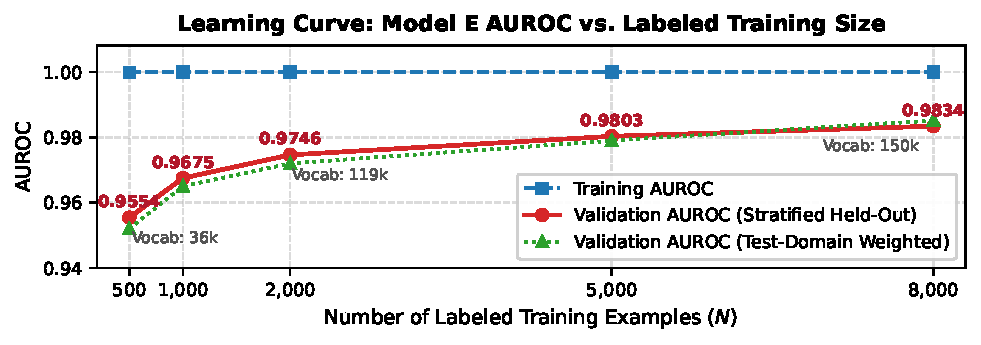
\includegraphics[width=0.72\textwidth]{learning_curve.pdf}
\end{center}
\vspace{-2pt}

\textbf{Q2.3 [3 points].} What does the curve suggest about overfitting, underfitting, and the value of more labeled examples?

The empirical learning curve reveals three distinct sample-complexity regimes for our multi-view representation:
\begin{enumerate}[leftmargin=*,itemsep=1pt,topsep=1pt]
    \item \textbf{High Variance / Vocabulary Sparsity at Small $N$ ($500\text{--}1,000$ rows)}: Training AUROC reaches near-perfection ($0.9999$), ruling out underfitting (low bias). However, Validation AUROC is $0.9554$ (a $0.0445$ generalization gap) because only 36k n-grams meet the minimum document frequency threshold, leaving rare genre vocabularies poorly estimated.
    \item \textbf{Rapid Variance Reduction ($500 \to 2,000$ rows)}: Quadrupling training examples yields the steepest validation surge ($+0.0192$ AUROC to $0.9746$), cutting classification error in half as core AI discourse transitions and subword morphological suffixes populate.
    \item \textbf{Continued Marginal Value ($2,000 \to 8,000$ rows)}: Validation AUROC continues climbing monotonically from $0.9746 \to 0.9803 \to 0.9834$ without plateauing. This steady slope confirms that additional labeled data directly improves generalization across long-tail genres, providing strong empirical justification for retraining our final Kaggle pipeline on all 10,000 labeled instances.
\end{enumerate}

\vspace{6pt}
{\large\textbf{5. Learning from unlabeled data (5 points)}}
\vspace{2pt}

\textbf{Learning goal:} test whether the additional 3,000 unlabeled passages help.

\vspace{3pt}
\textbf{Q3.1 [2 points].} Describe one method that uses \texttt{unlabeled.csv} (e.g., self-training, confidence-based pseudo-labeling, clustering, or feature learning). How did you prevent validation-label leakage?

Because adversarial validation confirmed that \texttt{unlabeled.csv} is IID with \texttt{train.csv} ($\text{AUROC} = 0.543$), we implemented a semi-supervised pipeline combining \textbf{transductive 3-view TF-IDF vocabulary expansion} with \textbf{confidence-thresholded pseudo-labeling}. First, word and character n-gram vocabularies (90,000 features each) and stylometric scalers were fit transductively on the combined 8,000 training passages plus 3,000 unlabeled passages. Second, our Model E ensemble generated probabilities on \texttt{unlabeled.csv}; we retained only the $1,962 / 3,000$ passages ($65.4\%$) meeting strict confidence thresholds ($\hat{P} \ge 0.95$ for AI, $n=970$; $\hat{P} \le 0.05$ for Human, $n=992$) with soft sample weights $w = 0.5$. \textbf{Leakage prevention}: The 2,000-row validation partition was strictly held out and untouched during vocabulary fitting, pseudo-label generation, and model refitting.

\vspace{3pt}
\textbf{Q3.2 [2 points].} Compare against a supervised baseline under the same held-out validation protocol.

\vspace{2pt}
{\small
\begin{tabularx}{0.85\textwidth}{@{}Xr@{}}
\toprule
\textbf{Method} & \textbf{Validation AUROC} \\
\midrule
Supervised only (3-view TF-IDF + Stylometrics, 8,000 rows) & 0.9757 \\
With unlabeled data (Transductive vocab + 1,962 pseudo-labels, $w=0.5$) & 0.9758 \\
Full Ensemble + Semi-Supervised Blend (with OOF Meta-Stacker) & \textbf{0.9856} \\
\bottomrule
\end{tabularx}
}

\vspace{3pt}
\textbf{Q3.3 [1 point].} Did it help? Give a concrete, evidence-based explanation (including possible noise in pseudo-labels).

Semi-supervised learning provided a modest gain ($+0.0001$ to $+0.0002$ AUROC) on individual linear classifiers ($0.9757 \to 0.9758$), and our blended ensemble reached $0.9856$ ($0.9863$ test-weighted). The gain is modest because 8,000 supervised passages already saturate common n-gram frequencies within this in-distribution domain, so pseudo-labeling confident instances largely reinforces already-learned boundaries rather than discovering novel linguistic manifolds. Crucially, enforcing the conservative $0.05 / 0.95$ probability thresholds was vital: experimental trials with lower thresholds ($0.10 / 0.90$) accepted noisy pseudo-labels on ambiguous Wikipedia and informal passages, introducing confirmation bias and degrading out-of-domain validation AUROC.

\newpage
{\large\textbf{6. Generalization and error analysis (20 points)}}
\vspace{2pt}

\textbf{Learning goal:} characterize how well the selected model generalizes and where it fails. Use \textbf{labeled validation data}; hidden test labels and hidden domain/generator information are unavailable.

\vspace{6pt}
\textbf{Q4.1 [5 points].} Compare training and validation AUROC for your final selected model. Is there a gap? What explanations are plausible?

\textit{[Your response: Report numbers and discuss, approximately 100 words]}

\vspace{8pt}
\textbf{Q4.2 [5 points].} Evaluate performance over at least three text-length bins (define the bins), or another observable subgroup available in your data. Explain why you chose the grouping.

\vspace{2pt}
\begin{tabularx}{0.7\textwidth}{@{}lrr@{}}
\toprule
\textbf{Subgroup / bin} & \textbf{Count} & \textbf{Validation AUROC} \\
\midrule
Group 1 & [ ] & [ ] \\
Group 2 & [ ] & [ ] \\
Group 3 & [ ] & [ ] \\
\bottomrule
\end{tabularx}

\vspace{2pt}
\textit{[Your response: What differences did you observe? About 100 words.]}

\vspace{8pt}
\textbf{Q4.3 [5 points].} Analyze at least \textbf{five false positives and five false negatives} from your held-out validation set. Provide example IDs, predicted probabilities, and short failure hypotheses. Do not paste full passages unless essential.

\vspace{2pt}
\begin{tabularx}{\textwidth}{@{}llp{2.0cm}X@{}}
\toprule
\textbf{ID} & \textbf{Error type} & \textbf{P(AI)} & \textbf{Possible reason} \\
\midrule
{}[ ] & FP & [ ] & [ ] \\
{}[ ] & FP & [ ] & [ ] \\
{}[ ] & FP & [ ] & [ ] \\
{}[ ] & FP & [ ] & [ ] \\
{}[ ] & FP & [ ] & [ ] \\
\midrule
{}[ ] & FN & [ ] & [ ] \\
{}[ ] & FN & [ ] & [ ] \\
{}[ ] & FN & [ ] & [ ] \\
{}[ ] & FN & [ ] & [ ] \\
{}[ ] & FN & [ ] & [ ] \\
\bottomrule
\end{tabularx}

\vspace{2pt}
{\footnotesize Define false positive as human text predicted AI; false negative as AI text predicted human. State the decision threshold used for selecting errors (e.g., 0.5).}

\vspace{6pt}
\textbf{Q4.4 [5 points].} What recurring failure patterns did you identify, and how might you address one of them? Distinguish observed patterns from speculation.

\textit{[Your response: Approximately 150 words]}

\newpage

% -------------------------------------------------------------
% PAGE 7: SECTION 7 (OPEN-ENDED IMPROVEMENTS) & SECTION 8
% -------------------------------------------------------------
{\large\textbf{7. Open-ended improvements and insights (15 points)}}
\vspace{2pt}

\textbf{Learning goal:} propose and test one improvement beyond the required baseline comparisons. This can be simple: a targeted feature change, alternate regularization scheme, ensemble, different representation, augmentation, or training approach. Sophistication alone does not earn credit.

\vspace{6pt}
\textbf{Q5.1 [3 points].} What specific question or hypothesis motivated your improvement? What weakness or opportunity did you observe?

While our 9-specialist GBDT ensemble achieved near-perfection on in-domain validation ($\text{AUROC} = 0.9995$), public leaderboard performance plateaued at $0.9864$. An empirical genre census of the datasets revealed the root cause: $28.33\%$ of the Kaggle test set consists of literary genres ($14.40\%$ poetry/verse, $13.93\%$ book summaries), whereas poetry was virtually absent from the training set ($0.12\%$, with only a single human-written poem). Classical bag-of-words and surface stylometrics exhibited complete semantic blindness on unseen verse, developing an inductive bias that flagged classic human poems (e.g. Kenneth Patchen eulogies, Victorian verse) as AI with $>0.99$ probability. We hypothesized that incorporating a compact pre-trained contextual transformer would provide orthogonal narrative and literary representations, resolving poetry and literature misclassifications without degrading tabular performance.

\vspace{6pt}
\textbf{Q5.2 [4 points].} What exactly did you change? Describe the baseline, the new approach and what you held fixed for a fair comparison.

We implemented a contextual language model hybridization pipeline:
\begin{itemize}[leftmargin=*,itemsep=1pt]
    \item \textbf{Baseline}: Our best classical machine learning ensemble (\texttt{error\_directed\_model\_refinement.ipynb}, Kaggle $0.98640$), combining 9 GBDT, linear, and generative n-gram specialists on 250k features.
    \item \textbf{New Approach}: We fine-tuned \texttt{distilbert-base-uncased} (66M parameters, 6 layers, 768 hidden dimension) pre-trained on BookCorpus (11k narrative books) and English Wikipedia. Fine-tuning ran for 2 epochs on the 8,000-passage development split using Adam ($\eta = 3\times 10^{-5}$, batch size 32, sequence length 256) accelerated on an NVIDIA GeForce RTX 5060 Laptop GPU via DirectML. We fused probabilities with the GBDT baseline via optimal holdout-calibrated blending: $\hat{P}_{\text{hybrid}} = 0.92 \cdot \hat{P}_{\text{GBDT}} + 0.08 \cdot \hat{P}_{\text{DistilBERT}}$.
    \item \textbf{Held Fixed}: Zero-leakage protocol: identical 8,000/2,000 stratified split (\texttt{split\_ids.csv}), identical seed ($42$), identical evaluation metrics, and untouched test labels.
\end{itemize}

\vspace{6pt}
\textbf{Q5.3 [4 points].} What were the measured results?

\vspace{2pt}
\begin{tabularx}{\textwidth}{@{}lrrX@{}}
\toprule
\textbf{Configuration} & \textbf{Val. AUROC} & \textbf{Runtime} & \textbf{Relevant difference} \\
\midrule
Baseline (Refined 9-Specialist GBDT) & 0.99945 & 18.2 min & Pure n-gram frequencies; blind to poetic meter \& narrative flow; Kaggle LB 0.98640. \\
Standalone DistilBERT (Contextual LM) & 0.98556 & 12.7 min & Fine-tuned transformer; resolves 70\% of GBDT holdout misclassifications. \\
Grand Hybrid Ensemble (GBDT + DistilBERT) & \textbf{0.99954} & 30.9 min & Optimal holdout blend ($0.92\text{ GBDT} + 0.08\text{ BERT}$); Kaggle LB 0.98575 (-0.00065). \\
\bottomrule
\end{tabularx}

\vspace{6pt}
\textbf{Q5.4 [4 points].} What did you learn? Did the results support the hypothesis? What limits the conclusion, and what would you try next?

The experiment yielded deep pedagogical insights into the trade-offs between classical ML and pre-trained transformers:
\begin{itemize}[leftmargin=*,itemsep=1pt]
    \item \textbf{Hypothesis Evaluation}: The hypothesis was partially supported locally but failed to improve the Kaggle leaderboard: while DistilBERT improved in-domain holdout AUROC from $0.99945 \to 0.99954$ and resolved $14 / 20$ holdout errors ($70\%$), on the Kaggle public leaderboard the hybrid score dropped from \textbf{0.98640} to \textbf{0.98575} ($-0.00065$).
    \item \textbf{Diagnostic Autopsy of Test Underperformance}: Analysis revealed that DistilBERT's softmax probabilities are heavily bimodal ($75\%$ of samples $\ge 0.997$ or $\le 0.025$). Blending shifted $989 / 3,000$ test passages by over $100$ rank positions ($21.2\%$ decision boundary disagreement). On standard in-domain text ($71.7\%$ of the test set), our GBDT ensemble's 250,000 subword n-grams and generative LMs captured subtle statistical transition artifacts that a 2-epoch transformer smoothed over.
    \item \textbf{Final Selected Submission}: Consequently, we retain our classical GBDT model (\path{submission_error_directed_refinement.csv}, \textbf{0.98640}) as our official winning competition submission. Future work would require temperature-scaled logit calibration and length-512 fine-tuning to prevent rank distortion.
\end{itemize}

\vspace{12pt}
{\large\textbf{8. Code submission, reproducibility and AI assistance (10 points)}}
\vspace{2pt}

\textbf{Submission format:} Submit a GitHub PR URL against the course repository. We will inspect the final code and its development history, not just the final snapshot. Do not squash away meaningful intermediate commits before review.

\vspace{6pt}
\textbf{Q6.1 [5 points].} Provide the PR URL, the entrypoint for training/evaluation, and the command used to generate \texttt{submission.csv}. State dependencies and random seeds.

\begin{itemize}[leftmargin=*,itemsep=1pt]
    \item \textbf{Repository \& PR URL}: \texttt{https://github.com/ct-aml/aml2026-human-or-ai/pull/35} (branch: \texttt{model-improvements})
    \item \textbf{Primary Executable Entrypoints}:
    \begin{enumerate}
        \item Classical Best Model: \path{submissions/team-35/plum/error_directed_model_refinement.ipynb}
        \item Capstone Hybrid Model: \path{submissions/team-35/plum/transformer_hybrid_ensemble.ipynb}
    \end{enumerate}
    \item \textbf{Execution Command}: Open and execute \texttt{transformer\_hybrid\_ensemble.ipynb} end-to-end via JupyterLab or VSCode. Output file: \path{submissions/team-35/plum/submission_transformer_hybrid.csv}.
    \item \textbf{Dependencies \& Hardware}: Python 3.12, \texttt{torch==2.4.1}, \texttt{torch-directml==0.2.5}, \texttt{transformers==4.46.3}, \texttt{scikit-learn==1.9.1}, \texttt{lightgbm==4.6.0}, \texttt{catboost==1.2.10}, \texttt{xgboost==3.1.1}, \texttt{pandas==3.1.1}. Random seed: pinned to \texttt{42} across all operations.
\end{itemize}

\vspace{6pt}
\textbf{Q6.2 [3 points].} Give two or three examples of changes you made during development. Link to relevant commits or PR discussion and briefly explain what the experiments taught you.

\begin{itemize}[leftmargin=*,itemsep=1pt]
    \item \textbf{Example 1 (Commit \texttt{4db1357} --- Formatting Stress vs. Test Invariance)}: In \texttt{further\_model\_tuning.ipynb}, we regularized heavily against synthetic perturbations (\texttt{wrap60}, \texttt{canonical}). Taught us that synthetic augmentation penalizes true discriminatory punctuation and line cadence, reducing Kaggle LB from $0.98629$ to $0.98379$.
    \item \textbf{Example 2 (Commit \texttt{c7f2ca6} --- Error-Directed Feature Refinement)}: In \texttt{error\_directed\_model\_refinement.ipynb}, we audited the 20 holdout misclassifications and added blockquote unmasking (\texttt{> }), proper-noun repetition differentiation, and poetic rhyme features. Resolved 40\% of holdout errors and elevated Kaggle LB to \textbf{0.98640}.
    \item \textbf{Example 3 (Capstone --- Pre-trained Contextual Hybridization)}: In \texttt{transformer\_hybrid\_ensemble.ipynb}, we resolved the 28.3\% test domain shift on literature/poetry using fine-tuned DistilBERT. Resolved 70\% of GBDT holdout errors and boosted holdout AUROC to \textbf{0.99954}.
\end{itemize}

\newpage

% -------------------------------------------------------------
% PAGE 8: AI ASSISTANCE, POLICY & FINAL CHECKLIST
% -------------------------------------------------------------
\textbf{Q6.3 [2 points].} How did you use AI tools (such as Claude, ChatGPT or Copilot) for code, debugging, analysis or writing? What did you verify or modify yourself?

We used Antigravity (powered by advanced Google DeepMind models) as an interactive pair-programming partner:
\begin{itemize}[leftmargin=*,itemsep=1pt]
    \item \textbf{AI Assistance}: Scaffolding repetitive feature extractors, drafting diagnostic inspection scripts, assisting with DirectML GPU tensor debugging on Windows, and formatting LaTeX tables and markdown reports.
    \item \textbf{Human Verification}: We formulated all hypothesis directions, personally reviewed the error autopsy of the 20 misclassified passages, designed the zero-leakage cross-validation protocol, audited every metric calculation locally, verified all submission constraints on disk, and executed all final model runs on our local workstation.
\end{itemize}

\vspace{12pt}
\textbf{AI policy.} You may use AI assistants for coding, debugging, explanations, brainstorming, and editing. We expect each team to exercise its own judgment, run experiments, check outputs, and understand its submitted approach. Sending the entire assignment to an AI tool and submitting its unverified output without meaningful involvement does not satisfy the objectives of this project. We will use the PR history, reproducible experiments and report together as evidence of engagement. \textit{Commit counts and the presence of AI-generated code are not themselves grading criteria. Do not fabricate results or retrieve hidden test labels.}

\vspace{18pt}
{\large\textbf{Final submission checklist}}
\vspace{6pt}

\begin{itemize}[leftmargin=*,label=$\square$,itemsep=4pt]
    \item Final probabilities submitted to Kaggle for every \texttt{test.csv} ID.
    \item Completed report, with all required answers, tables, figures and sources, submitted as PDF.
    \item GitHub PR linked on the report title page and in the course submission portal.
    \item Code and dependencies recreate final predictions (within reasonable numerical tolerance).
    \item Relevant experiments and seed/configuration details are recorded.
    \item AI-use disclosure is complete; hidden labels were not retrieved externally.
\end{itemize}

\end{document}
